%%%%%%%%%%%%%%%%%%%%%%%%%%%%%%%%%%%%%%%%%
% Dreuw & Deselaer's Poster
% LaTeX Template
% Version 1.0 (11/04/13)
%
% Created by:
% Philippe Dreuw and Thomas Deselaers
% http://www-i6.informatik.rwth-aachen.de/~dreuw/latexbeamerposter.php
%
% This template has been downloaded from:
% http://www.LaTeXTemplates.com
%
% License:
% CC BY-NC-SA 3.0 (http://creativecommons.org/licenses/by-nc-sa/3.0/)
%
%%%%%%%%%%%%%%%%%%%%%%%%%%%%%%%%%%%%%%%%%

%----------------------------------------------------------------------------------------
%	PACKAGES AND OTHER DOCUMENT CONFIGURATIONS
%----------------------------------------------------------------------------------------

\documentclass[final,hyperref={pdfpagelabels=false}]{beamer}

\usepackage[orientation=portrait,size=a0,scale=1.4]{beamerposter} % Use the beamerposter package for laying out the poster with a portrait orientation and an a0 paper size

\usetheme{I6pd2} % Use the I6pd2 theme supplied with this template

\usepackage[english]{babel} % English language/hyphenation

\usepackage{amsmath,amsthm,amssymb,latexsym} % For including math equations, theorems, symbols, etc

%\usepackage{times}\usefonttheme{professionalfonts}  % Uncomment to use Times as the main font
%\usefonttheme[onlymath]{serif} % Uncomment to use a Serif font within math environments

\boldmath % Use bold for everything within the math environment

\usepackage{booktabs} % Top and bottom rules for tables

\graphicspath{{figures/}} % Location of the graphics files

\usecaptiontemplate{\small\structure{\insertcaptionname~\insertcaptionnumber: }\insertcaption} % A fix for figure numbering

%----------------------------------------------------------------------------------------
%	TITLE SECTION 
%----------------------------------------------------------------------------------------

\title{\huge Feature Enhancement of Amandroid, an Open Source Static Analyzer for the Security Vetting of Android Applications.} % Poster title

\author{Author:Shiva Bhusal, Supervisor: Dr. Sankardas Roy} % Author(s)

\institute{Department of Computer Science} % Institution(s)

%----------------------------------------------------------------------------------------
%	FOOTER TEXT
%----------------------------------------------------------------------------------------
%% Any footer information will be here. 

\newcommand{\leftfoot}{} % Left footer text

\newcommand{\rightfoot}{} % Right footer text

%----------------------------------------------------------------------------------------

\begin{document}

\addtobeamertemplate{block end}{}{\vspace*{2ex}} % White space under blocks

\begin{frame}[t] % The whole poster is enclosed in one beamer frame

\begin{columns}[t] % The whole poster consists of two major columns, each of which can be subdivided further with another \begin{columns} block - the [t] argument aligns each column's content to the top

\begin{column}{.02\textwidth}\end{column} % Empty spacer column

\begin{column}{.465\textwidth} % The first column

%----------------------------------------------------------------------------------------
%	The Android Ecosystem
%----------------------------------------------------------------------------------------

\begin{block}{The Android Ecosystem}

\begin{itemize}
\item Android is the most popular mobile operating system in the world.
\item Android has caught up to windows in terms of the internet use. (Businessinsider, 2017)
\item The Android Ecosystem consists of three major players: the users, the publishers and the app Store agency. 
\item Android Ecosystem is not void of malicious apps. 
\end{itemize}

\begin{figure}
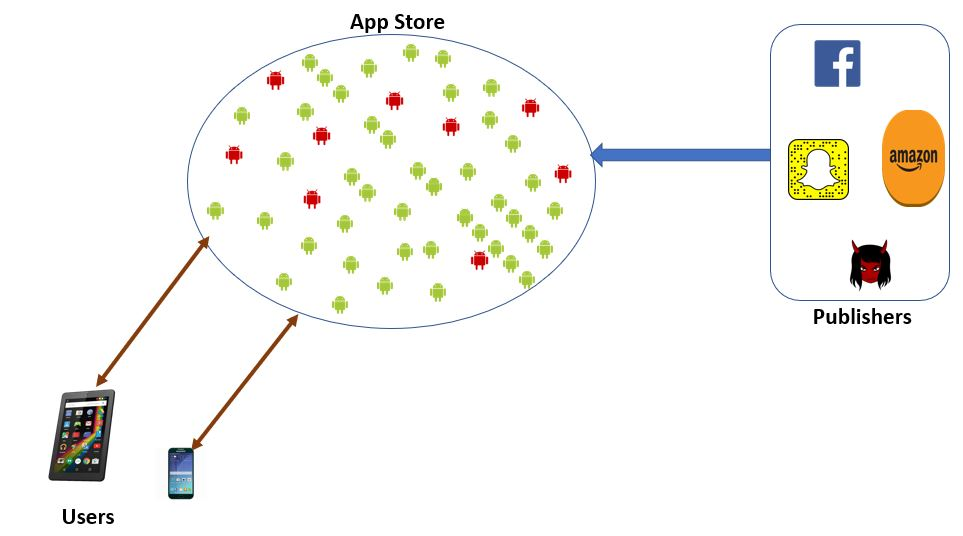
\includegraphics[width=0.8\linewidth]{AndroidEcoSystem.JPG}
\caption{Android Ecosystem}
\end{figure}

\end{block}

%----------------------------------------------------------------------------------------
%	The Art of Static Analysis
%----------------------------------------------------------------------------------------
            
\begin{block}{The Art Of Static Analysis}

\begin{itemize}
\item Static Analysis is the way of analyzing an application without actually running it. 
\item Static analysis is useful in Android Ecosystem to detect \alert {malicious apps} before users install in their machine or even before they are uploaded to the App store. 
\item Static analysis is not perfect.It is not void of false positives and false negatives. 
\end{itemize}

\end{block}

\begin{block}{Amandroid: A Tool Of The Trade}

\begin{itemize}
\item Amandroid is an open source static analyzer used for the security vetting of Android Apps. 
\item The idea behind Amandroid is to perform data flow, control flow and the data dependence analysis for each of the components of an Android App.
\item This helps detect possibilities of malicious activities such as:  
\begin{itemize}
\item Sensitive data leakage.
\item Data injection. 
\item Misuse of sophisticated APIs.  
\end{itemize}
\end{itemize}

\begin{figure}
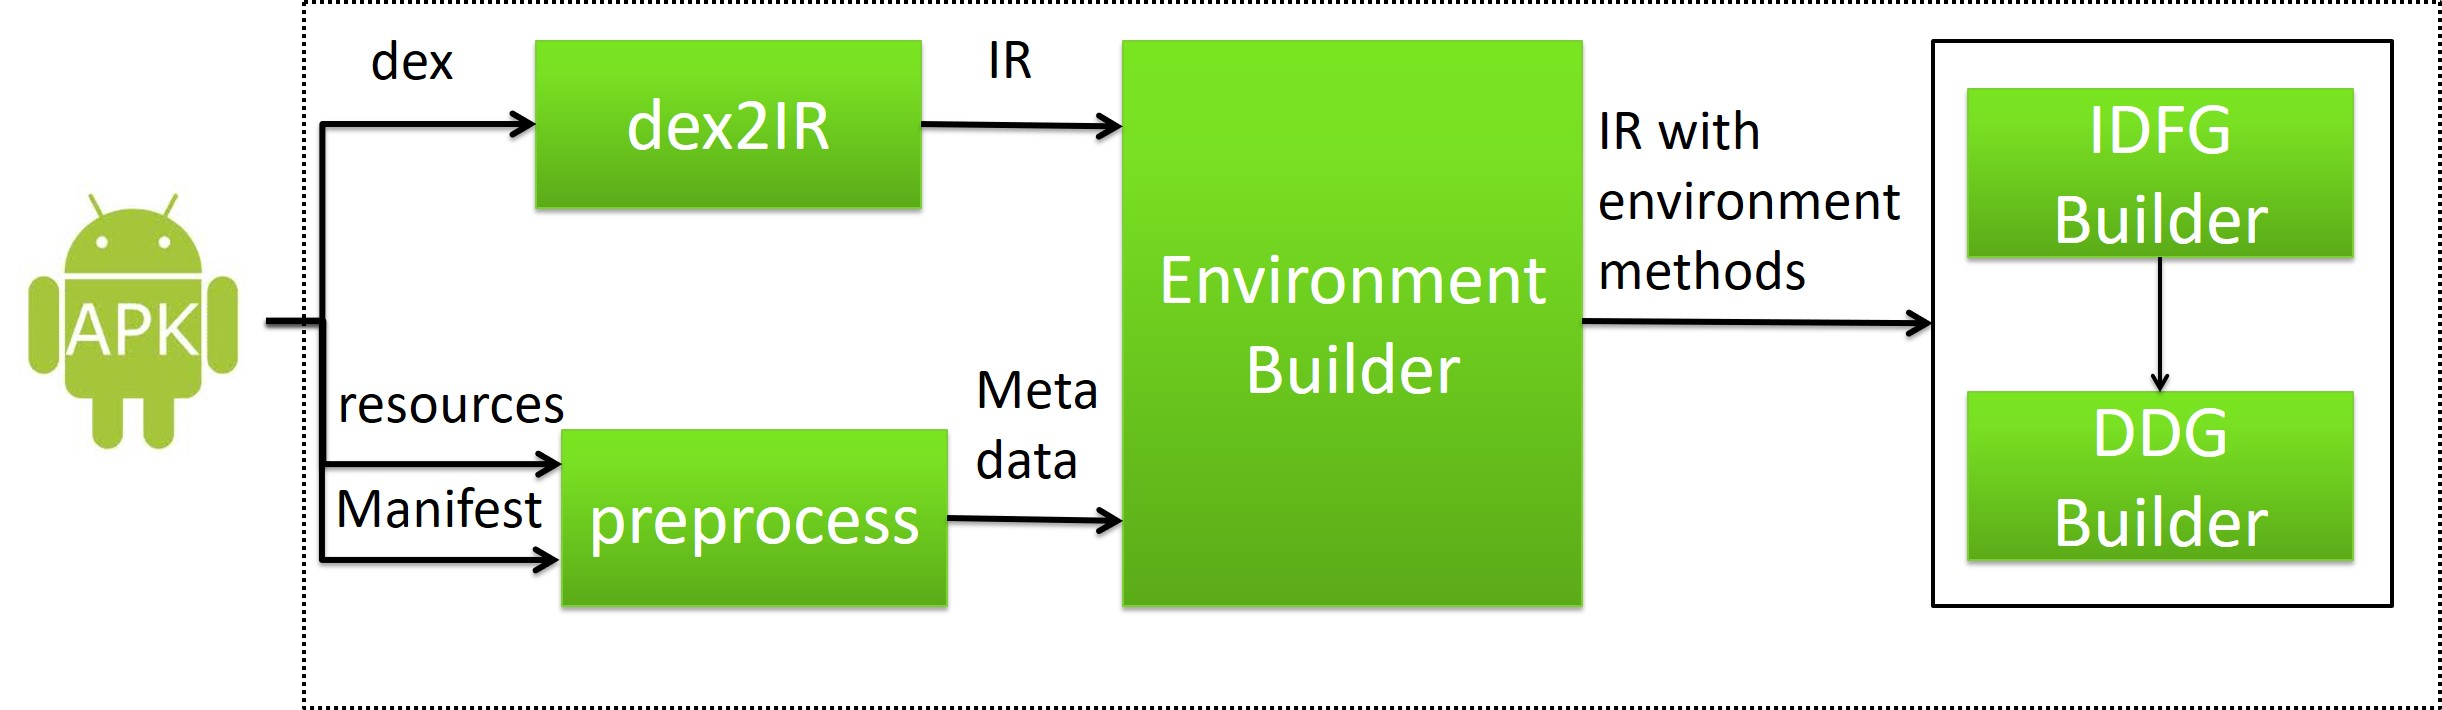
\includegraphics[width=0.8\linewidth]{Amandroid.jpg}
\caption{Amandroid block diagram( Wei Et. Al)}
\end{figure}

\begin {itemize}
\item Amandroid can be downloaded in the form of a jar file, and can be used to detect malicious activities in any APKs.
\end{itemize}
\end{block}

%----------------------------------------------------------------------------------------
%	Problem Statement
%----------------------------------------------------------------------------------------

\begin{block}{Problem Statement}
\begin{itemize}
\item Attackers are implementing newer techniques to create malicious apps. 
\item Every static analysis tools have to be updated and enhanced to detect the newer forms of malicious activities. 
\item Currently, Amandroid doesn't have plugins to detect potential malicious activities such as:
\begin{itemize}
\item Blackmailing users through the misuse of LockScreen. 
\item Dynamic loading of Hexcode from network or the asset folder of the Android app. Etc.
\end{itemize}
\item The motto of this work is how the features of Amandroid can be enhanced so that it detects  newer forms of potential malicious activities. 

\end{itemize}

\end{block}

\end{column} % End of the first column

\begin{column}{.03\textwidth}\end{column} % Empty spacer column
 
\begin{column}{.465\textwidth} % The second column

%----------------------------------------------------------------------------------------
%	A motivating example: LockScreen
%----------------------------------------------------------------------------------------

\begin{block}{Motivating example I : LockScreen}
\begin{itemize}
\item \textbf{Malicious Symptoms:}
    \begin{itemize}
    \item Once the app is installed, it covers the entire screen of the Android device. 
    \item The victim is not able to close the malicious App or access any other apps already installed in their device. 
    \item The app may consist of some blackmailing information. 
  \end{itemize}
\item \textbf{The lockScreen detector plugin:} 
\begin{itemize}
\item Checks for the presence of signature that can be malicious. 
\item Checks for a particular value of the parameter in the call statement which confirms the presence of LockScreen.
\end{itemize}
\end{itemize}  
\end{block}

%-----------------------------------------------

\begin{block}{Motivating Example II:  Dynamic loading}
\begin{itemize}
\item \textbf{Malicious Symptoms:}
    \begin{itemize}
    \item Loads Dalvik Bytecode from asset folder or network. 
    \item The hidden Dalvik Bytecode has malicious intent. 
  \end{itemize}
  \item \textbf{Why attackers use dynamic loading ?}
    \begin{itemize}
    \item Because it's difficult for an static analysis application to analyze the source code dynamically loaded from another source. 
  \end{itemize}
\item \textbf{The Dynamic loading detector plugin:} 
\begin{itemize}
\item Checks for the presence of signature that can be malicious. 
\item Checks for the use of DexClassLoader class. 
\end{itemize}
\end{itemize}  
\end{block}

\begin{block}{Testing and Verification}
\begin{itemize}
\item Both the LockScreen and DynamicLoading detector plugins were tested using \textbf {ScalaTests.} 
\item Both the plugins passed 5 different test cases. 
\end{itemize}
\end{block}

\begin{block}{Experimental Results}
\begin{itemize}
\item 
\item 
\end{itemize}
\end{block}

%%%%%%%
% Future Works 
%%%%%%%
\begin{block}{Future Works}

\begin{itemize}
\item Writing more plugins to detect newer tricks used by attackers. 
\item Using Machine Learning techniques to detect malicious and benign apps.  
\begin{itemize}
\item Result of each plugin becomes one feature for the classifier. 
\end{itemize}
\end{itemize}
\begin{figure}
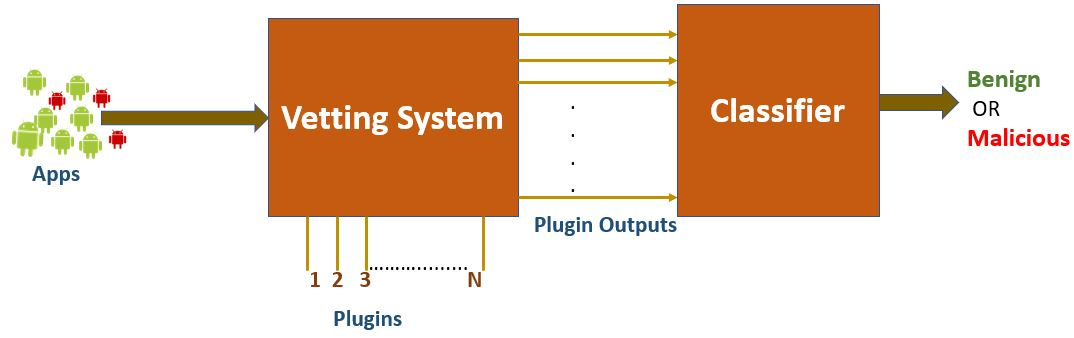
\includegraphics[width=0.8\linewidth]{futureWorks.JPG}
\caption{Machine Learning based Classifier}
\end{figure}


\end{block}

%----------------------------------------------------------------------------------------
%	REFERENCES
%----------------------------------------------------------------------------------------

\begin{block}{References}
\begin{enumerate}
\item Amandroid: ACM CCS 2014, \href{http://pag.arguslab.org/argus-saf}{http://pag.arguslab.org/argus-saf} 
\end{enumerate}

%%Uncomment it to load Refernces from sample.bib         
%%\nocite{*} % Insert publications even if they are not cited in the poster
%%\small{\bibliographystyle{unsrt}
%%\bibliography{sample}}

\end{block}

%----------------------------------------------------------------------------------------
%	ACKNOWLEDGEMENTS
%----------------------------------------------------------------------------------------

\begin{block}{Acknowledgments}

\begin{itemize}
\item Fengguo Wei, Dewan Chaulagain, Steven Arzt. 
\end{itemize}
\end{block}

\end{column} % End of the second column

\begin{column}{.015\textwidth}\end{column} % Empty spacer column

\end{columns} % End of all the columns in the poster

\end{frame} % End of the enclosing frame

\end{document}